\documentclass[../../labo_tp5_main.tex]{subfiles}

\begin{document}

%capítulo
\section{Ejercicio 6}

En Argentina, el espectro de FM se divide en 7 categor\'ias (de la A a la G) seg\'un su radio de servicio, es decir hasta d\'onde la potencia de la estaci\'on se mantiene dentro de los 48$\frac{dB\mu}{m}$.

\begin{figure}[H]
	\centering
	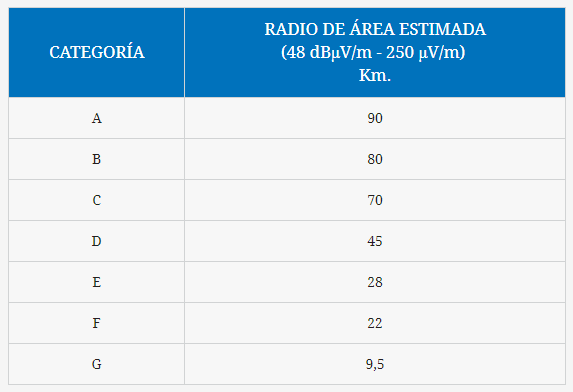
\includegraphics[scale=0.6]{imagenes/categorias.png}
	\caption{Categor\'ias de emisoras FM}
\end{figure}

\end{document}
